\documentclass[tikz,border=6pt]{standalone}
\usepackage{tikz}

\begin{document}
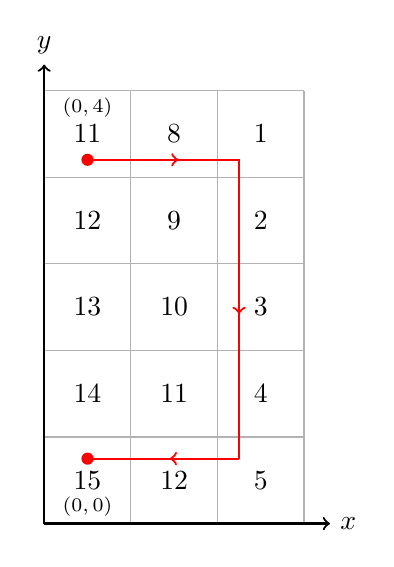
\begin{tikzpicture}[scale=1.1]

  % -------- INPUT --------
  \def\Nx{3}             % number of columns
  \def\Ny{5}             % number of rows

  % Draw grid
  \draw[thin,gray!60] (0,0) grid (\Nx,\Ny);

  % Column drawing function
  \newcommand{\drawcolumn}[3]{%
      % Bottom row
      \node at (#1+0.5,0.5) {\number#2};
      % Higher rows: subtract y
      \foreach \y in {1,...,\numexpr#3-1} {
          \newcount\tmp
          \tmp=#2
          \advance\tmp by -\y
          \node at (#1+0.5,\y+0.5) {\number\tmp};
      }%
  }

  % Draw all columns
  \drawcolumn{0}{15}{\Ny}
  \drawcolumn{1}{12}{\Ny}
  \drawcolumn{2}{5}{\Ny}

  % Mark start and end
  \fill (0.5,4.8) node {\scriptsize $(0,4)$};
  \fill (0.5,0.2) node {\scriptsize $(0,0)$};

  % Axes
  \draw[->,thick] (0,0) -- (\Nx+0.3,0) node[right] {$x$};
  \draw[->,thick] (0,0) -- (0,\Ny+0.3) node[above] {$y$};

  % ---------- Path visualization ----------
  % First right move
  \draw[red,thick]    (0.5,4.2) -- (2.26,4.2);
  \draw[red,thick,->] (0.5,4.2) -- (1.55,4.2); % arrow

  % Down move
  \draw[red,thick]    (2.25,4.2) -- (2.25,0.74);
  \draw[red,thick,->] (2.25,4.2) -- (2.25,2.42); % arrow

  % Left move
  \draw[red,thick]    (2.25,0.75) -- (0.5,0.75);
  \draw[red,thick,->] (2.25,0.75) -- (1.45,0.75); % arrow

  % Mark the path nodes
  \foreach \x/\y in {0.5/4.2,0.5/0.75} {
      \fill[red] (\x,\y) circle (2pt);
  }

\end{tikzpicture}
\end{document}
